Uno de los principales problemas de hacer ingeniería de rendimiento para software en la nube es que no existen aplicaciones de referencia que hayan ganado popularidad o cuyo desarrollo se encuentre activo. A pesar de esto y de su reciente adopción, la industria ha empezado a reconocer casos de uso en donde las aplicaciones \emph{serverless} encajan mejor. Amazon Web Services(AWS)\cite{serverless-architecture-patterns} reconoce cinco patrones de uso predominantes en su servicio AWS Lambda:
\begin{enumerate}
    \item Procesamiento de datos dirigidos por eventos.
    \item Aplicaciones Web.
    \item Aplicaciones móviles e Internet las cosas (IoT).
    \item Ecosistemas de aplicaciones \emph{serverless}.
    \item Flujos de trabajo dirigidos por eventos.
\end{enumerate}
 
Uno de las aplicaciones más comunes en \emph{serverless} es desencadenar acciones luego de que ocurre un evento (1), por ejemplo luego de la modificación de un registro en una base de datos o bien luego de que se publica un mensaje en una cola de mensajería. Esto puede provocar que se active una función Lambda\footnote{En la plataforma AWS Lambda } que toma como entrada el evento recién publicado para su posterior procesamiento. Este estilo de caso de uso encaja bien en ambientes híbridos: ambientes en donde tecnologías \emph{serverless} se aprovechan para realizar funciones específicas dentro de una aplicación (o aplicaciones) más grande.

AWS ha publicado una serie de arquitecturas de referencia\cite{aws-lambda-ref-arch} para su plataforma FaaS, AWS Lambda. Dentro de estas arquitecturas se destaca el caso de uso de un manejador de imágenes (\emph{Image Handler})\cite{aws-lambda-image-handler}. 

\begin{figure}[h]
  \centering
  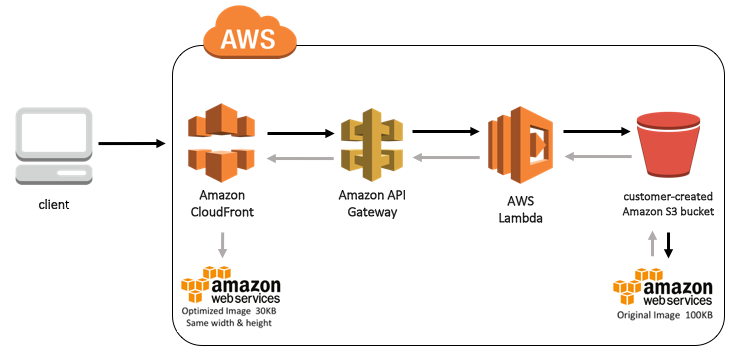
\includegraphics[width=15cm]{serverless-image-handler-architecture}
  \caption[Arquitectura del manejador de imágenes]{Arquitectura del manejador de imágenes. Tomado de \protect\cite{aws-lambda-image-handler}}
  \label{fig:serverless-image-handler-architecture}
\end{figure}

\section{\emph{Manejador de imágenes}} \label{sec:manejador-imagenes-1}
Sitios Web con imágenes grandes pueden experimentar tiempos de carga prolongados, es por esto que los desarrolladores proporcionan diferentes versiones de cada imagen para que se acomoden a distintos anchos de banda o diseños de página. Para brindar tiempos de respuesta cortos y disminuir el costo de la optimización, manipulación y procesamiento de las imágenes, AWS propone un manejador de imágenes \emph{serverless}, al cual se le pueda delegar tal trabajo como una función Lambda sobre la plataforma FaaS.


A continuación se describe la arquitectura de la figura \ref{fig:serverless-image-handler-architecture}:
\begin{enumerate}
    \item Amazon CloudFront provee una capa de \emph{cache} para reducir el costo del procesamiento de la imagen
    \item Amazon API Gateway brinda acceso por medio de HTTP a las funciones Lambda
    \item AWS Lambda obtiene la imagen de un repositorio de Amazon Simple Storage Service (Amazon S3) y por medio de la implementación de la función se retorna una versión modificada de la imagen al API Gateway
    \item El API Gateway retorna una nueva imagen a CloudFront para su posterior entrega a los usuarios finales
\end{enumerate}

Cabe mencionar que, en este contexto, una versión modificada de una imagen será cualquier imagen que haya presentado algún tipo de alteración con respeto de una imagen original como, por ejemplo, cambios de tamaño, color, metadatos, etc.

\subsection{Manejador de imágenes para SPE} \label{sec:manejador-imagenes-spe}
Para este estudio se proponemos implementar una variación del manejador de imágenes de la sección \ref{sec:manejador-imagenes-1}, que se muestra en la figura \ref{fig:serverless-image-handler-architecture-spe}.

\begin{figure}[h]
  \centering
  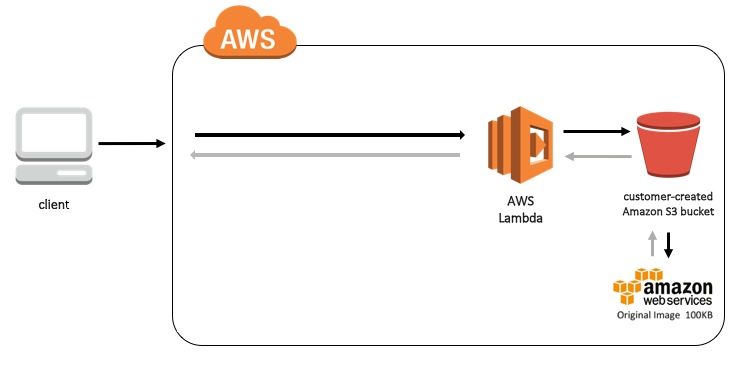
\includegraphics[width=15cm]{serverless-image-handler-architecture-spe}
  \caption[Arquitectura del manejador de imágenes propuesto para el estudio]{Arquitectura del manejador de imágenes propuesto para el estudio.}
  \label{fig:serverless-image-handler-architecture-spe}
\end{figure}

Se han dejado por fuera intencionalmente el AWS CloudFront y el AWS API Gateway. La razón de esto es porque se pretende ejercitar la función Lambda directamente. Se implementará una función Lambda que entregue a partir de una solicitud de redimensionamiento de una imagen almacenada, otra con dimensiones diferentes producida ``al vuelo'' como respuesta a la solicitud. Por ejemplo, si la imagen original mide 500 pixeles de ancho y alto, entregar una con dimensiones de 100 pixeles de ancho y alto. 

Las actividades involucradas en el proceso de redimensionamientos de imágenes se muestran en la figura \ref{fig:serverless-image-handler-architecture-workflow}
\begin{enumerate}
    \item Se envía una solicitud de redimensionamiento de imagen en formato \texttt{JSON} a la función Lambda con los datos acerca de la localización de la imagen y su nuevo tamaño.
    \item La solicitud de redimensionamiento llega a la función Lambda.
    \item La función Lambda solicita al servicio de almacemiento AWS S3 la imagen.
    \item AWS S3 entrega a la función Lambda la imagen solicitada.
    \item La función Lambda inicia el redimensionamiento de la imagen de acuerdo a los parámetros solicitados.
    \item La nueva imagen modificada se entrega al cliente(s).
\end{enumerate}

\begin{figure}[h]
  \centering
  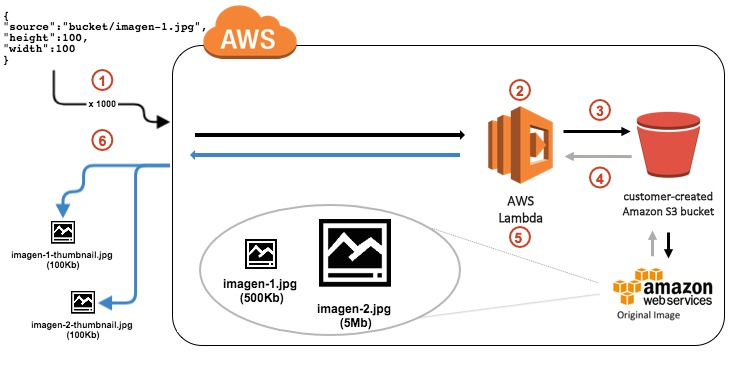
\includegraphics[width=17cm]{serverless-image-handler-architecture-workflow-2}
  \caption[Carga de trabajo sugerida para el manejador de imágenes]{Carga de trabajo sugerida para el manejador de imágenes}
  \label{fig:serverless-image-handler-architecture-workflow}
\end{figure}


A la función Lambda se le realizarán pruebas con imágenes de entrada de distinto tamaño y cargas de trabajo variables para evaluar su comportamiento bajo estos escenarios. Se desea observar el impacto de las pruebas en el tiempo de respuesta de la función. Los resultados obtenidos a partir de estas pruebas van a servir como un punto de referencia para experimentos futuros, como los que se indican en la Sección \ref{sec:experimentos-propuestos}. La figura \ref{fig:serverless-image-handler-architecture-workflow} muestra una sugerencia de dos posibles cargas de trabajo: 

\begin{enumerate}
    \item 100 solicitudes de cambio de tamaño de una imagen grande. En la figura \ref{fig:serverless-image-handler-architecture-workflow}, \texttt{imagen-2.jpg} de tamaño de 5Mb, representa una imagen grande.
    \item 100 solicitudes de cambio de tamaño de una imagen pequeña. En la figura \ref{fig:serverless-image-handler-architecture-workflow}, \texttt{imagen-1.jpg} de tamaño menor o igual a 500Kb, representa una imagen pequeña.
\end{enumerate}

En principio las cargas de trabajo generadas serían \emph{cerradas}, lo que quiere decir que una solicitud se ejecuta solamente hasta que la anterior se termina. Esto ayudará en principio a tener mejor trazabilidad de lo que ocurre con la función.

\paragraph{¿Por qué este caso de uso se considera relevante?}
A continuación se listan las características que hacen este caso de uso representativo e interesante:
\begin{itemize}
    \item Sencillo de entender e implementar: se cuenta únicamente con una función la cual lleva a cabo una tarea muy específica.
    \item Popular: sigue un patrón de procesamiento dirigido por eventos y, como se señala en \cite{serverless-architecture-patterns}, este es uno de los más populares que se ha empezado a adoptar para aplicaciones \emph{serverless}. Otra de las razones de la popularidad de este caso de uso es que permite a los desarrolladores crear una unidad de instalación independiente y especializada para el manejo de imágenes, liberando así a sus servidores y aplicaciones del manejo de las peticiones y lógica asociadas a estas.
    \item Replicable en otros proveedores de servicios en la nube: varias de las arquitecturas de referencia para \emph{serverless} propuestas por Amazon, están compuestas por herramientas y servicios muy propios de su plataforma, lo cual hace muy difícil su reproducibilidad utilizando otros proveedores. Aunque en principio este trabajo plantea ser elaborado en la plataforma FaaS de Amazon Web Services, AWS Lambda, otros proveedores de servicios (ver sección \ref{sec:proveedores-faas}) en la nube cuentan con sus propias plataformas de FaaS y de almacenamiento, lo cual permitiría replicar lo aquí propuesto en ellos.
    \item Replicable en los lenguajes de programación soportados por plataformas FaaS: actualmente JavaScript, Java (y lenguajes basados en la \emph{Java Virtual Machine}), Python, C\# y Go son los principales lenguajes de programación soportados por las plataformas FaaS. El caso de uso propuesto, no presenta ningún tipo de característica que lo ate a un lenguaje de programación en particular. En todos ellos se cuentan con bibliotecas para manejo de imágenes tanto de forma nativa como por medio de soluciones de terceros. 
\end{itemize}


\section{Implementación del \emph{manejador de imágenes}}
Existen soluciones disponibles que se pueden estudiar para implementar un manejador de imágenes. Amazon proporciona dos ejemplos que siguen la arquitectura de la figura \ref{fig:serverless-image-handler-architecture}:
\begin{enumerate}
    \item \textbf{{serverless-image-resizing}}\footnote{\url{https://github.com/amazon-archives/serverless-image-resizing}}: escrita en lenguaje JavaScript. Utiliza el modulo \emph{sharp}\footnote{\url{https://github.com/lovell/sharp}} de NodeJS para aplicar operaciones de conversión en imágenes tales como redimensionamiento, rotación y corrección gamma.
    \item \textbf{{serverless-image-handler}}\footnote{\url{https://github.com/awslabs/serverless-image-handler}}: escrita en lenguaje Python. Hace uso del paquete \emph{Thumbor}\footnote{\url{http://thumbor.org}} de código abierto para realizar operaciones de redimensionamiento, rotación, recorte y aplicación de filtros en imágenes.
\end{enumerate}

A pesar que Amazon recomienda el uso de \emph{serverless-image-handler} sobre \emph{serverless-image-resizing}, ambas soluciones siguen un patrón sumamente similar en su codificación e instalación. 

Otro ejemplo de una función en la nube encargada de ofrecer un servicio de redimensionamiento en imágenes, es la \emph{Course\_LambdaResizer}, una función lambda usada como referencia en el curso \emph{``Serverless API on AWS for Java developers''} ofrecido en el sitio Web Udemy\footnote{\url{https://www.udemy.com/serverless-api-aws-lambda-for-java-developers}}. Esta función está escrita en lenguaje Java y utiliza la biblioteca \emph{imgscalr}\footnote{\url{https://github.com/rkalla/imgscalr}} para redimensionar imágenes.

Para este estudio, se implementó una función escrita en lenguaje Java. Esto motivado principalmente por la compatibilidad de este lenguaje con las herramientas para monitoreo de aplicaciones y extracción de modelos de rendimiento, Kieker y PMX respectivamente.

\subsection{Función Lambda: \emph{Image-Handler} (IM-Simple)}\label{sec:image-handler}
La función Lambda creada para este estudio lleva por nombre \emph{Image-Handler}. El código fuente y documentación relacionada con la misma se encuentra disponible en GitHub.com, en el repositorio de código: \url{https://github.com/seminario-dos/image-handler}. El punto de entrada de la función Lambda es la clase \texttt{ImageHandler.java}. Esta función se encarga de realizar tres operaciones para procesar una solicitud de redimensionamiento de imagen:

\begin{enumerate}
    \item Procesar la solicitud de redimiensionamiento (la entrada) que viene dada en formato JSON. Esta solicitud de redimensionamiento contiene entre otras cosas:
    \begin{itemize}
        \item El nombre de la imagen original que reside en el servicio Amazon S3.
        \item Los parámetros de altura y ancho a los que se desea redimensionar la imagen original.
    \end{itemize}
    \item Obtener la imagen del servicio Amazon S3 y posteriormente aplicar la operación de redimiensionamiento sobre la misma de acuerdo a los parámetros de altura y ancho especificados en la solicitud de redimensionamiento.
    \item Tomar la imagen redimensionada, codificarla en \texttt{Base64} y escribir el resultado en el flujo(\emph{stream}) de salida de la función Lambda.
\end{enumerate}
 
Un extracto de la clase \texttt{ImageHandler.java} se muestra en el listado \ref{lst:lambda-1}. En la línea \texttt{22} se procesa el evento de entrada que viene dado en formato JSON. Como resultado de esto se entrega un objeto \texttt{ImageRequest} el cual contiene la información de la solicitud de la imagen que se desea redimensionar y que se encuentra alojada en el servicio Amazon S3.

En la línea \texttt{24} se llama al servicio \texttt{ImageService} con el fin de obtener la imagen   original (de acuerdo a la información presente en el \texttt{ImageRequest} proporcionado) y se aplica la operación de redimensionamiento.

Por último, en la línea \texttt{26}, \texttt{ImageHandlerResponseWriter.writeResponse()} toma la nueva imagen, con nuevas dimensiones de alto y ancho, la codifica en \texttt{Base64} y escribe el resultado en el \emph{stream} de salida de la función. 

\begin{lstlisting}[linewidth=16.5cm, caption={Clase \texttt{ImageHandler.java}}, label={lst:lambda-1}]
public class ImageHandler implements RequestStreamHandler {

    private static final AppConfig APP_CONFIG;
    private final AppConfig appConfig;

    static {
        APP_CONFIG = AppConfig.getInstance();
    }

    public ImageHandler() {
        this(APP_CONFIG);
    }

    public ImageHandler(AppConfig appConfig) {
        this.appConfig = appConfig;
    }

    @Override
    public void handleRequest(InputStream inputStream, 
                              OutputStream outputStream, 
                              Context context) throws IOException {
        ImageRequest imageRequest = 
            this.inputEventParser().processInputEvent(inputStream);
        InputStream imageResized = 
            this.imageService().getImageFrom(imageRequest);
        this.imageHandlerResponseWriter()
            .writeResponse(imageResized, outputStream, imageRequest);
    }

    private InputEventParser inputEventParser() {
        return this.appConfig.getInputEventParser();
    }

    private ImageService imageService() {
        return this.appConfig.getImageService();
    }

    private ImageHandlerResponseWriter imageHandlerResponseWriter() {
        return this.appConfig.getImageHandlerResponseWriter();
    }
}    
\end{lstlisting}


Las funciones Lambda en AWS reciben como entrada un objeto JSON. Este objeto puede contener distintos campos dependiendo del servicio que haya invocado previamente la ejecución de la función Lambda. Debido a que la función \emph{Image-Handler} pretende ser invocada por medio de solicitudes \texttt{HTTP}, esta se configuró para que trabajara en conjunto con el servicio \texttt{API Gateway}. Dentro de este servicio se creó un recurso Web que entrega solicitudes de tipo \texttt{HTTP GET} a la función Lambda para su posterior procesamiento.

En términos generales, cada vez que una solicitud \texttt{HTTP GET} ingresa al \texttt{API Gateway} con el siguiente formato:\\ \texttt{https://\{host\}/image/\{image\}?width=\{value\}\&height=\{value\}}\\ se tomarán el nombre de la imagen original que viene en el parámetro \texttt{image} y los parámetros de ancho y alto, \texttt{width} y \texttt{height} respectivamente, y se pasarán como parámetros de entrada a la función Lambda como parte de un objeto JSON. Este objeto JSON contiene otros campos que dan a conocer a la función Lambda información acerca de la solicitud \texttt{HTTP}.

\paragraph{Ejemplo:} para la siguiente solicitud \texttt{HTTP}:
\begin{verbatim}
GET https://{host}/images/original-pic.jpg?width=50&height=66
\end{verbatim}

\noindent \texttt{API Gateway} produce el objeto JSON listado en \ref{lst:lambda-api-gateway-input}. A pesar que el objeto JSON incluye otros campos, para efectos del \emph{Image-Handler} solamente tres de ellos serán utilizados:
\begin{enumerate}
    \item \texttt{pathParameters}: contiene el nombre de la imagen original a ser redimensionada.
    \item \texttt{isBase64Encoded}: señala si la solicitud necesita ser codificada en \texttt{Base64} o no. 
    \item \texttt{queryStringParameters}: bajo esta propiedad se listan los parámetros de ancho(\texttt{width}) y alto(\texttt{height}).
\end{enumerate}


\begin{lstlisting}[caption={Clase \texttt{ImageHandler.java}}, label={lst:lambda-api-gateway-input}]
{
  "headers": {
    "Accept": "*/*",
    "User-Agent": "HTTPie/1.0.2",
    "Connection": "keep-alive",
    "X-Forwarded-Proto": "http",
    "Host": "localhost:3000",
    "Accept-Encoding": "gzip, deflate",
    "X-Forwarded-Port": "3000"
  },
  "pathParameters": {
    "image": "original-pic.jpg"
  },
  "path": "/images/original-pic.jpg",
  "isBase64Encoded": true,
  "requestContext": {
    "accountId": "123456789012",
    "path": "/images/{image+}",
    "resourceId": "123456",
    "stage": "prod",
    "requestId": "c6af9ac6-7b61-11e6-9a41-93e8deadbeef",
    "identity": {
      "cognitoIdentityPoolId": null,
      "accountId": null,
      "caller": null,
      "apiKey": null,
      "sourceIp": "127.0.0.1",
      "cognitoAuthenticationType": null,
      "cognitoAuthenticationProvider": null,
      "userArn": null,
      "userAgent": "Custom User Agent String",
      "user": null
    },
    "resourcePath": "/images/{image+}",
    "httpMethod": "GET",
    "extendedRequestId": null,
    "apiId": "1234567890"
  },
  "resource": "/images/{image+}",
  "httpMethod": "GET",
  "body": null,
  "queryStringParameters": {
    "width": "50",
    "height": "66"
  },
  "stageVariables": null
}
\end{lstlisting}

\subsubsection{Principales interacciones dentro de \emph{Image-Handler}}
La figura \ref{fig:secuencia-image-handler} muestra las principales interacciones que lleva a cabo la función \emph{Image-Handler}. Tanto las acciones como los actores involucrados, concuerdan con lo descrito en la Sección \ref{sec:image-handler} aunque, a diferencia de lo descrito allí, aquí se presenta la clase \texttt{S3Dao} que es la que se encarga de buscar y traer la imagen original del servicio Amazon S3. 
\begin{figure}[h]
  \centering
  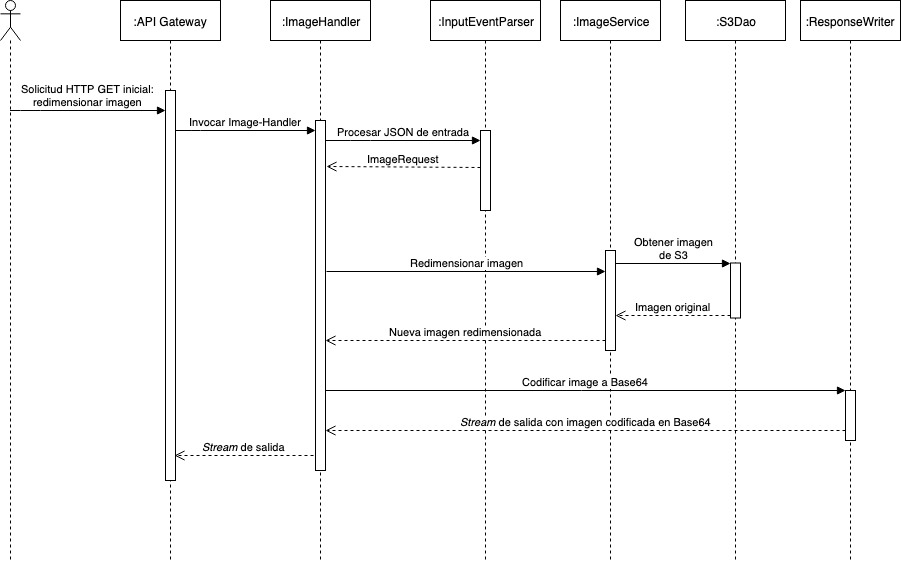
\includegraphics[width=16.5cm]{secuencia-image-handler}
  \caption{Secuencia de acciones llevadas a cabo por \emph{Image-Handler}}
  \label{fig:secuencia-image-handler}
\end{figure}

\subsection{Versiones alternas de \emph{Image-Handler}}

Aparte de la versión original de \emph{Image-Handler}, se crearon dos versiones alternas con el fin de instrumentalizar el código fuente para la extracción y generación de un modelo en PCM a partir, y para la obtención de mediciones del rendimiento. 

En la primer version, el código se modificó para generar rastros del rendimiento de la función Lambda y extraer a partir de estos un modelo de rendimiento en PCM. La segunda versión fue modificada para generar rastros de rendimiento pero, a diferencia de la versión anterior, los datos obtenidos en esta versión fueron de mayor utilidad para afinar las estimaciones de rendimiento de los componentes involucrados en la función.

\subsubsection{Versión instrumentalizada para Kieker y PMX (IM-KP)} \label{sec:image-handler-kieker-pmx}

Uno de los principales objetivos de este trabajo es el de obtener un modelo de rendimiento a partir 
del código en ejecución de una función en la nube. A pesar que, el modelo de rendimiento puede ser creado por los diseñadores e implementadores sin necesidad de una herramienta que ayude a su extracción, el uso de una herramienta especializada para esto contribuye a la generación de un modelo que pueda incluir mayores niveles de detalle en cuanto a la estructura y estimaciones del comportamiento de un software. Además, debido a que se están dando los primeros pasos en el campo del modelado y simulación de rendimiento basado en componentes, es preferible delegar tareas de extracción y estimaciones a una herramienta(s) con el fin de aprender de lo resultados obtenidos e ir introduciendo cambios paulatinamente; la creación manual de modelos de rendimiento puede llegar a ser muy compleja, consumir mucho tiempo y ser propensa a errores. 

Para lograr esto, se seleccionaron dos herramientas, Kieker y PMX, las cuales en conjunto proporcionan un marco de trabajo por medio del cual se puede obtener mediciones del rendimiento de una aplicación y luego, a partir de estas, extraer un modelo de rendimiento basado en PCM. La selección de estas herramientas y el enfoque de medición y extracción de modelos de rendimiento se seleccionó luego de estudiar el \emph{enfoque de ingeniería de rendimiento declarativo} propuesto en \cite{Walter:2018:TDP:3185768.3185777}.


%Kieker se utiliza para el estudiar el comportamiento del rendimiento del sistema a partir de las entradas/rastros que se registran en una bitácora. Creada y mantenida por el grupo de ingeniería de software de la Universidad de Kiel en conjunto con el grupo de sistemas de software de la Universidad de Stuttgart, Kieker se define como una herramienta para monitoreo del rendimiento y análisis dinámico de aplicaciones y se desarolló como parte de las actividades de enseñanza e investigación de ambas universidades. Otras instituciones académicas y de la industria también han realizado contribuciones.

Kieker se utiliza para el estudiar el comportamiento del rendimiento del sistema a partir de las entradas/rastros que se registran en una bitácora. Kieker ofrece adaptadores de monitoreo (\emph{monitoring adapters}) escritos en lenguaje Java (también ofrece adaptadores en otros lenguajes). Los dos principales componentes de Kieker son: \texttt{Kieker.Monitoring} y \texttt{Kieker.Analysis}. \texttt{Kieker.Monitoring} es el responsable de la instrumentación del código, recolección de datos y registro(\emph{logging}). El componente \texttt{Kieker.Analysis} es el responsable de leer, analizar y visualizar los datos monitoreados.

En esta versión de \emph{Image-Handler} se modificó el código original para generar registros del rendimiento de la ejecución de la función utilizando las bibliotecas proporcionadas por Kieker, utilizando como referencia lo especificado en el manual de usuario de Kieker\cite{kieker-user-guide}. Se crean objetos de tipo \texttt{OperationExecutionRecord} los cuales son los que contienen la información acerca del rendimiento de una invocación sobre alguna parte del código.  En el listado \ref{lst:image-handler-kieker} se puede ver un extracto del código de la función instrumentalizada para que genere objetos\\ \texttt{OperationExecutionRecord}.

Adicionalmente se configuró la biblioteca para que publique los objetos\\ \texttt{OperationExecutionRecord} a modo eventos a una cola de mensajería \emph{Java Message Service} (JMS), en lugar de una bitácora local.

\begin{lstlisting}[caption={Extracto de la clase \texttt{ImageHandler.java} instrumentalizada con Kieker}, label={lst:image-handler-kieker}]
public class ImageHandlerKieker implements RequestStreamHandler {
    private static final IMonitoringController MONITORING_CONTROLLER;
    static {
        MONITORING_CONTROLLER = MonitoringController.getInstance();
    }
    .
    .
    .
    
    @Override
    public void handleRequest(InputStream inputStream, OutputStream outputStream, Context context) throws IOException {

        final long tin = MONITORING_CONTROLLER.getTimeSource().getTime();
        handleRequestInternal(inputStream, outputStream, context);
        final long tout = MONITORING_CONTROLLER.getTimeSource().getTime();
        final OperationExecutionRecord e = new OperationExecutionRecord("public void "+ this.getClass().getName()+".handleRequest(InputStream, OutputStream, Context)",
                OperationExecutionRecord.NO_SESSION_ID,
                OperationExecutionRecord.NO_TRACE_ID,
                tin, tout,
                InetAddress.getLocalHost().getHostName(),
                0,
                0);
        MONITORING_CONTROLLER.newMonitoringRecord(e);
    }
    .
    .
    .
}    
\end{lstlisting}


\emph{Performance Model Extractor} (PMX), es una herramienta que automatiza la extracción de modelos de rendmiento a partir de mediciones. PMX utiliza como entrada las bitácoras basadas en Kieker y es capaz de crear modelos basados en \emph{Palladio Component Model} a partir de estas. 

%Esta es una herramienta creada y mantenida por el grupo de ingeniería de software de la Universidad Würzburg en Alemania.

%En conjunto, Kieker y PMX, proporcionan un marco de trabajo por medio del cual se puede obtener mediciones del rendimiento de una aplicación y luego, a partir de estas, extraer un modelo de rendimiento basado en PCM. La selección de estas herramientas y el enfoque de medición y extracción de modelos de rendimiento se seleccionó luego de estudiar el \emph{enfoque de ingeniería de rendimiento declarativo} propuesto en \cite{Walter:2018:TDP:3185768.3185777}.
%
%Esta versión de \emph{Image-Handler} fue la que se utilizó para obtener un modelo de rendimiento en \emph{Palladio Component Model} a partir de la bitácora basada en Kieker que se generó luego de múltiples invocaciones a la función Lambda. El proceso de extracción se detalla en la Sección \ref{sec:estrategia-de-extraccion-de-modelo}.

Los aspectos relacionados con la estrategia de cómo se obtuvo un modelo de rendimiento a partir de las bitácoras de Kieker y PMX se dan a conocer en la Sección \ref{sec:estrategia-de-extraccion-de-modelo}.

\subsubsection{Versión instrumentalizada para AWS X-Ray (IM-XRay)}
La principal motivación detrás de esta nueva versión de \emph{Image-Handler} es la de contar con datos del rendimiento de la función Lambda que no pudieron llegar a ser estimados durante el proceso de extracción del modelo utilizando PMX. En la Sección \ref{sec:estrategia-de-extraccion-de-modelo} se brindan los detalles de lo observado durante el proceso de extracción del modelo con PMX y en dónde encajan los resultados arrojados por esta nueva versión en el modelo.
 
Para esta versión, Se siguió un enfoque similar al de la Sección \ref{sec:image-handler-kieker-pmx} pero en lugar de utilizar la biblioteca de Kieker, se utilizó la biblioteca AWS SDK (\emph{Software Development Kit, SDK}) para crear las trazas y \emph{subsegmentos} de trazas, que son vistas más específicas del comportamiento de la aplicación. Con el uso AWS X-Ray se busca: 
\begin{enumerate}
    \item Obtener datos específicos del rendimiento de la función.
    \item Averiguar si las nuevas mediciones logran brindar información acerca de la infraestructura AWS Lambda y su impacto en la ejecución de \emph{Image-Handler}.
    \item Exportar los datos de rendimiento a algún formato conocido para su manipulación.
\end{enumerate}

Se modificó la función \emph{Image-Handler} para que puede generar trazas de AWS X-Ray en los mismos puntos en el código en los que se agregó la instrumentalización para Kieker. Un extracto de este código se muestra en el listado \ref{lst:image-handler-xray}. Cada invocación a las operaciones de procesamiento de la entrada, redimensionamiento y entrega de la respuesta se realizan utilizando el método \texttt{AWSRay.createSubsegment}.

\begin{lstlisting}[caption={Extracto de la clase \texttt{ImageHandler.java} instrumentalizada con AWS X-Ray}, label={lst:image-handler-xray}]
public class ImageHandlerXRay implements RequestStreamHandler {
    .
    .
    .
    @Override
    public void handleRequest(InputStream inputStream, OutputStream outputStream, Context context) throws IOException {
        ImageRequest imageRequest = AWSXRay.createSubsegment("input event", new Function<Subsegment, ImageRequest>() {
            @Override
            public ImageRequest apply(Subsegment subsegment) {
                return inputEventParser().processInputEvent(inputStream);
            }
        });

        InputStream imageResized = AWSXRay.createSubsegment("resize event", new Function<Subsegment, InputStream>() {
            @Override
            public InputStream apply(Subsegment subsegment) {
                return imageService().getImageFrom(imageRequest);
            }
        });

        AWSXRay.createSubsegment("write response", () -> {
            imageHandlerResponseWriter().writeResponse(imageResized, outputStream, imageRequest);
        });
    }
    .
    .
    .
}
\end{lstlisting}


\begin{figure}[h]
  \centering
  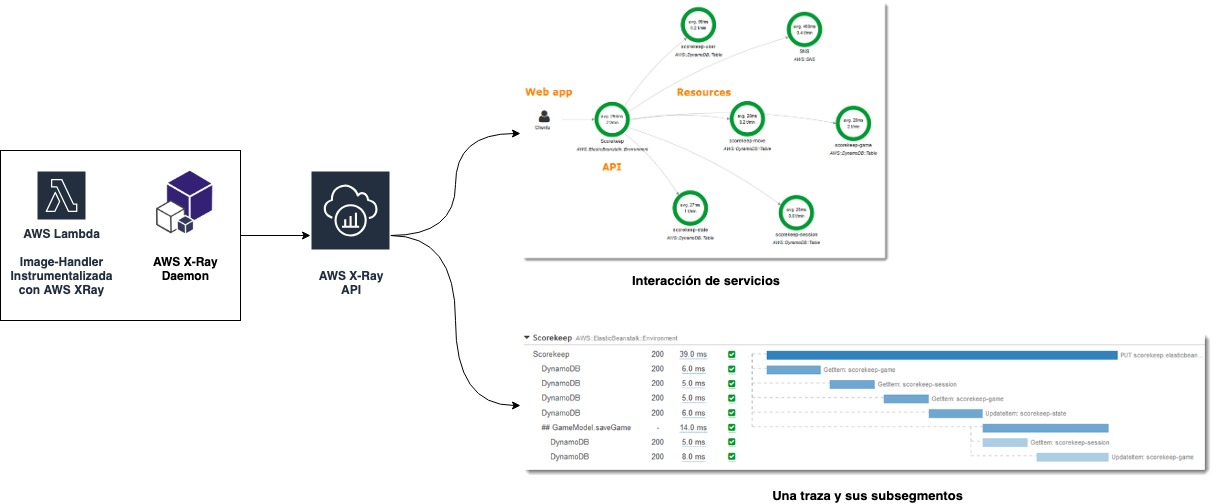
\includegraphics[width=17cm]{image-handler-xray}
  \caption{\emph{Image-Handler} publicando eventos de rendimiento al servicio AWS X-Ray}
  \label{fig:image-handler-xray}
\end{figure}

En la figura \ref{fig:image-handler-xray} se muestran los principales involucrados en la generación de trazas de rendimiento en AWS X-Ray. A la función \emph{Image-Handler} se le agrega la biblioteca de AWS X-Ray para crear las trazas. Estas trazas se envían al servicio AWS X-Ray que es el recolecta estas trazas y con base en ellas se pueden obtener mapas de la interacción de los servicios que componen la función y desgloces de los subsegmentos que componen la traza.


\section{Estrategia de extracción de modelo de rendmiento para \emph{Image-Handler}} \label{sec:estrategia-de-extraccion-de-modelo}
 
Debido a que las funciones Lambda se ejecutan en contenedores que son tanto inaccesibles como efímeros para los diseñadores e implementadores, y, sobre los cuales no se tiene ningún control, estrategias tradicionales en donde se crean bitácoras en la misma computadora en donde se ejecuta la aplicación y se van monitoreando utilizando alguna herramienta especializada o simplemente mediante \emph{Secure Socket Channel}(\texttt{SSH}) deben ser replanteadas. Para este tipo de software, se hace necesario registrar los eventos asociados al comportamiento del rendimiento en una computadora o servicio externo en el cual se tenga control para acceder a los resultados y manipularlos.

Para lograr extraer un modelo PCM a partir de las bitácoras de Kieker, se llevaron a cabo las siguientes actividades:
\begin{enumerate}
    \item Creación de la versión Image-PK (Sección \ref{sec:image-handler-kieker-pmx}): Versión de \emph{Image-Handler} instrumentalizar el código fuente con las bibliotecas de Kieker para generar bitácoras del rendimiento de la función.    
%    de acuerdo con su manual de usuario\cite{kieker-user-guide}. Se crean objetos de tipo \texttt{OperationExecutionRecord} los cuales contienen información acerca del rendimiento de una invocación sobre alguna parte del código, y luego estos objetos se publican a una cola de mensajería para su posterior tratamiento. En el listado \ref{lst:image-handler-kieker} se puede ver un extracto del código de la función instrumentalizada para que genere objetos  \texttt{OperationExecutionRecord}.
    \item Provisionar una nueva máquina virtual en AWS la cual se va a:
    \begin{itemize}
        \item Ejecutar una cola JMS.
        \item Ejecutar una aplicación consumidora de mensajes de la cola JMS.
        \item Almacenar la bitácora de registros de rendimiento de la función Lambda.
    \end{itemize}


    \item Configurar la biblioteca de Kieker para señalar que la publicación de los registros de rendimiento de la función se hagan a través de la cola JMS en la máquina virtual del punto \#2.
    \item Creación de una aplicación consumidora de mensajes para que una vez que arriben los mensajes a la cola JMS, esta procese los mensajes de la cola y los almacene en una bitácora.
\end{enumerate}

%\begin{lstlisting}[caption={Extracto de la clase \texttt{ImageHandler.java} instrumentalizada con Kieker}, label={lst:image-handler-kieker}]
%public class ImageHandlerKieker implements RequestStreamHandler {
%    private static final IMonitoringController MONITORING_CONTROLLER;
%    static {
%        MONITORING_CONTROLLER = MonitoringController.getInstance();
%    }
%    .
%    .
%    .
%    
%    @Override
%    public void handleRequest(InputStream inputStream, OutputStream outputStream, Context context) throws IOException {
%
%        final long tin = MONITORING_CONTROLLER.getTimeSource().getTime();
%        handleRequestInternal(inputStream, outputStream, context);
%        final long tout = MONITORING_CONTROLLER.getTimeSource().getTime();
%        final OperationExecutionRecord e = new OperationExecutionRecord("public void "+ this.getClass().getName()+".handleRequest(InputStream, OutputStream, Context)",
%                OperationExecutionRecord.NO_SESSION_ID,
%                OperationExecutionRecord.NO_TRACE_ID,
%                tin, tout,
%                InetAddress.getLocalHost().getHostName(),
%                0,
%                0);
%        MONITORING_CONTROLLER.newMonitoringRecord(e);
%    }
%    .
%    .
%    .
%}    
%\end{lstlisting}

% generara registros del rendimiento de la ejecución utilizando las bibliotecas proporcionadas por Kieker, de acuerdo con su manual de usuario\cite{kieker-user-guide}. En lugar de publicar los registros en alguna bitácora local, los registros del rendimiento se publican en una cola \emph{Java Message Service}(JMS). Una vez que arriban los mensajes a la cola JMS, otra aplicación empieza a consumir los mensajes y los va almacenando en una bitácora. 

La figura \ref{fig:image-handler-kieker} muestra los involucrados en el proceso de publicación de mediciones de rendimiento del código de \emph{Image-Handler} hacia una bitácora externa.

Una vez que la función Lambda se ejercitó y se haya obtenido una bitácora de Kieker, se toma esta bitácora como entrada para PMX, con el fin de obtener una instancia de PCM. Esto se aprecia en la figura \ref{fig:image-handler-pmx}. Se espera que, al utilizarse datos de mediciones directas del rendimiento de la función Lambda, PMX pueda generar una instacia de PCM que sea confiable y de la que se puedan obtener simulaciones que representativas del comportamiento de la función Lambda.

\begin{figure}[h]
  \centering
  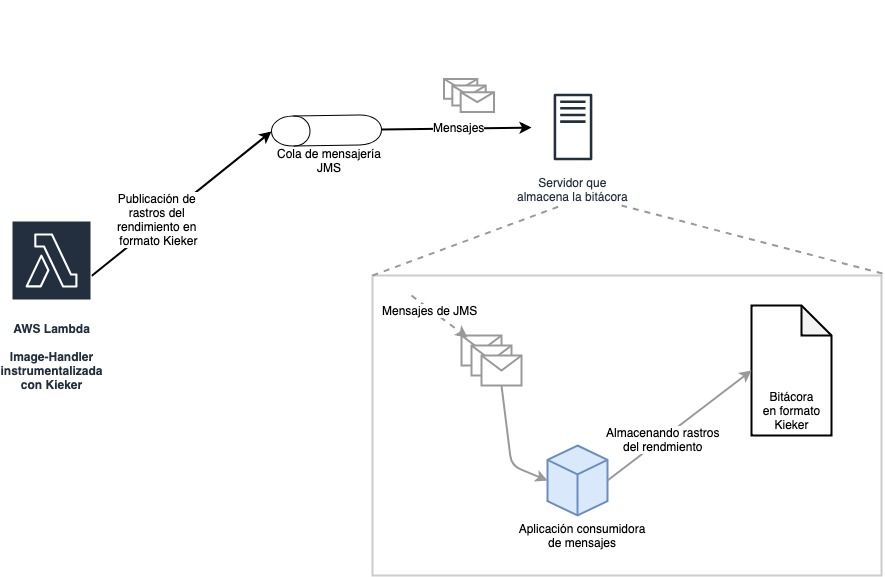
\includegraphics[width=17cm]{image-handler-kieker}
  \caption{Publicando mediciones del rendimiento de la función Lambda.}
  \label{fig:image-handler-kieker}
\end{figure}

\begin{figure}[h]
  \centering
  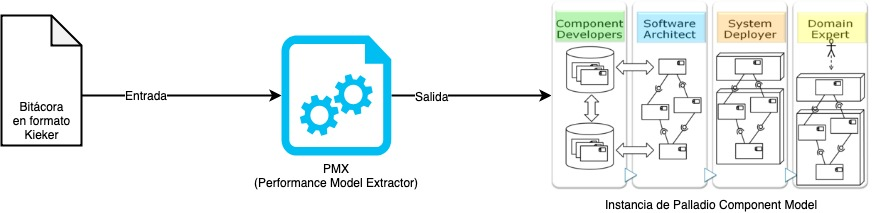
\includegraphics[width=17cm]{image-handler-pmx}
  \caption{Convirtiendo una bitácora de Kieker a una instancia de PCM por medio de PMX.}
  \label{fig:image-handler-pmx}
\end{figure}

\subsubsection{Versión instrumentalizada para AWS X-Ray}\label{sec:image-handler-xray}
Una actividad recurrente durante el modelado y simulación de arquitecturas de software, es la del afinamiento del modelo. Esta tarea es necesaria para que el modelo en cual se está trabajando pueda llegar a convertirse una representación cercana del comportamiento de un software en escenarios reales. 

Durante el trabajo con el modelo PCM obtenido en la Sección \ref{sec:image-handler-kieker-pmx} se notó que las estimaciones hechas por PMX no correspondían al comportamiento observado y que el esfuerzo necesario para obtener estas estimaciones a partir de las bitácoras de Kieker iba a ser grande, principalmente porque el formato de las bitácoras de Kieker incluye muchos más datos que solo las estimaciones de rendimiento y porque se empezó a tener la sensación de que estos datos de alguna u otra forma no estaban ``contando toda la historia'' de lo que estaba pasando con la función Lambda. Por ejemplo, las datos de rendimiento de Kieker no podían explicar tiempos de retraso que se observaban al inicio de la ejecución de la función Lambda y, sin esos datos, se podía llegar a generar un modelo poco preciso.

Por esta razón se comenzó a explorar herramientas alternativas para obtener mediciones del rendimiento de la función Lambda y se elegió Amazon X-Ray\footnote{\url{https://aws.amazon.com/xray/}} para este fin. AWS XRay ayuda a los desarrolladores a analizar y depurar aplicaciones en producción distribuidas, tal y como lo son las basadas en arquitecturas de microservicios. Con AWS X-Ray se puede ver cómo es que la aplicación y sus servicios asociados se están ejecutando para identificar y resolver problemas de rendimiento y errores en general.

AWS X-Ray recolecta datos de las solicitudes que hacen a cada uno de los servicios de la aplicación y los agrupa en unas unidades llamadas trazas(\emph{traces}). Luego, utilizando estas trazas, es posible ver mapas de la interacción de los servicios, latencias y meta datos para analizar el comportamiento o identificar problemas.




\section{Diseño Experimental}
En esta sección se detallan los experimentos realizados para validar si el modelo y la simulaciones sobre el mismo, logran dar caracterizaciones relevantes del comportamiento de la función \emph{Image Handler} en distintos escenarios. 

\subsection{Utilizando \emph{Image-Handler} para redimensionar imágenes de distintos tamaños}
Este es el caso que se menciona en la Sección \ref{sec:manejador-imagenes-spe} y se muestra en la figura \ref{fig:serverless-image-handler-architecture-workflow}. Se probó la función Lambda con dos imágines: una de tamaño pequeño ($\sim$100Kb) y otra de tamaño grande ($\sim$5Mb). El objetivo es comprobar cómo los distintos tamaños de las imágenes influyen en el tiempo de respuesta de la función.

Intuitivamente, se espera que, cuando se hagan solicitudes de redimensionamiento de imágenes de mayor tamaño tomen mayor tiempo en ser procesadas y que lo contrario suceda con las imágenes de menos tamaño. Los resultados obtenidos brindan una referencia inicial para saber cómo es que los componentes de software asociados al redimensionamiento trabajan y qué posibles mejoras podrían realizarse.

Las cargas de trabajo para este experimento son de tipo \emph{cerrada}, lo que quiere decir que una solicitud se ejecuta solamente hasta que la anterior se termina. Esto va orientado a tener mejor trazabilidad de lo que ocurre con la función.

\subsubsection{Ejercitando la función Lambda con solicitudes de redimensionamiento en una imagen pequeña($\sim$100Kb)}

Este, al ser el primer experimento realizado, sentó las bases del marco de trabajo en modelaje y simulación que se aplicaron en otros experimentos. 

Se utilizó la siguiente configuración para la ejecución del experimento:

\begin{enumerate}
    \item Se utilizó una imagen de tamaño de 19Kb y de 295 pixeles de ancho y alto.
    \item La función \emph{Image-Handler} se ejercitó con una carga de trabajo \emph{cerrada} de 100 solicitudes de redimensionamiento para convertir la imagen del punto \#1 a una imagen de 50 pixeles de ancho y 60 de alto.
    \begin{enumerate}
        \item En primera instancia, las 100 solicitudes se hicieron usado la versión de la función \emph{Image-Handler} instrumentalizada con Kieker (Sección \ref{sec:image-handler-kieker-pmx}), para obtener una bitácora con las operaciones realizada
        \item Posteriormente, esta bitácora fue procesada por PMX para obtener una instancia de PCM.
    \end{enumerate}
    \item Una vez obtenido la instancia de PCM, se ejecutó otra carga de trabajo \emph{cerrada} de 100 solicitudes de redimensionamiento pero esta vez utilizando la versión de la función \emph{Image-Handler} instrumentalizada con AWS X-Ray (Sección \ref{sec:image-handler-xray}). Esto para obtener métricas más detalladas sobre el uso de la función y así para afinar las estimaciones de los componentes que conforman la instancia de PCM.
    \begin{enumerate}
        \item Una vez obtenidas estas mediciones, se realizaron análisis de frecuencias para determinar la distribución de las cargas de trabajo en cada componente.
    \end{enumerate}
    \item Se realizaron simulaciones sobre la instancia de PCM utilizando el motor de simulaciones provisto por \emph{Palladio Workbench}. 
    \item Se ejecutó una carga de trabajo \emph{cerrada} de 100 solicitudes de redimensionamiento utilizando la versión original de la función \emph{Image-Handler}.
    \item Por último se compararon y analizaron los resultados del punto \#4 y \#5 para determinar si, de acuerdo a lo obtenido, las simulaciones hechas sobre el modelo lograban caracterizar el rendimiento de la función Lambda.
\end{enumerate}


Como resultado del trabajo llevado a cabo en el punto \#2, se obtuvieron los componentes mostrados en la figura \ref{fig:image-handler-pcm-model}. En PCM a este diagrama se le conoce como diagrama de repositorio.

\begin{landscape}
\begin{figure}[h]
  \vspace*{-3cm}  
  \centering
  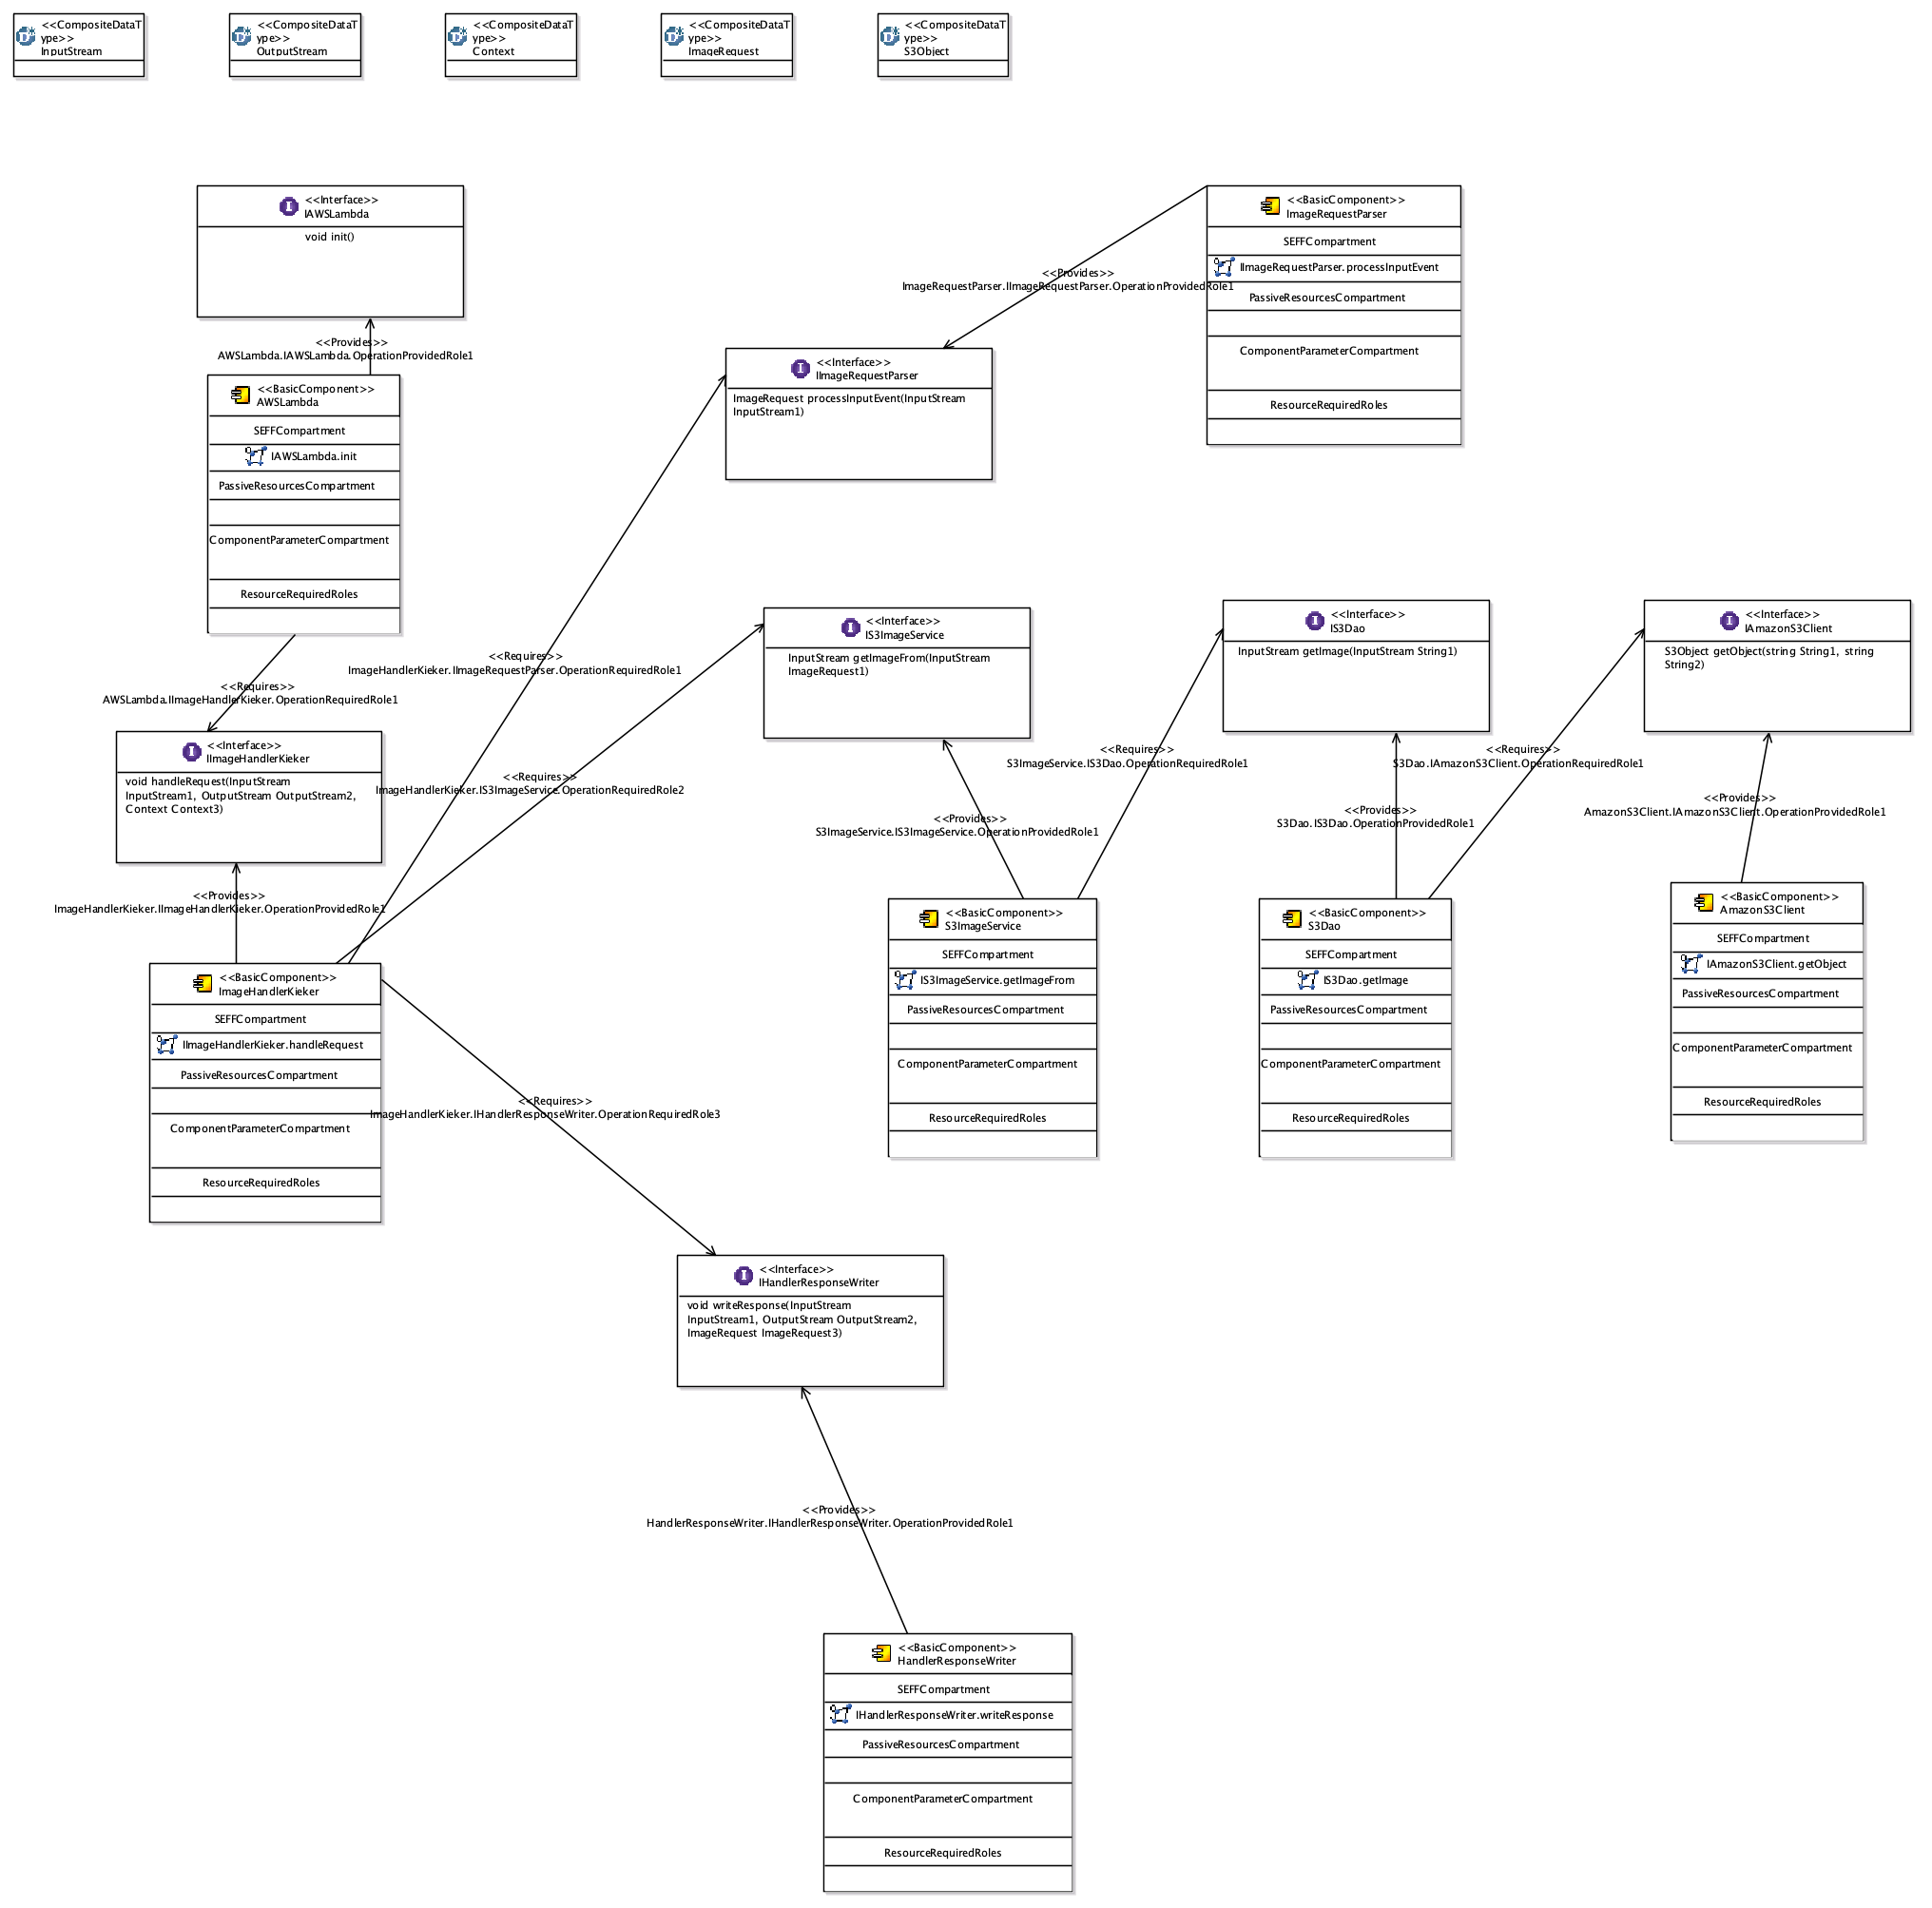
\includegraphics[width=20cm]{image-handler-extracted-repository-diagram.png}
  \caption{\emph{Image-Handler} publicando eventos de rendimiento al servicio AWS X-Ray}
  \label{fig:image-handler-pcm-model}
\end{figure}
\end{landscape}

A partir de la bitácora proporcionada como entrada, PMX logró identificar 6 componentes principales:
\begin{itemize}
    \item \texttt{ImageHandlerKieker}: El punto de entrada de la función.
    \item \texttt{ImageRequestParser}: Encargado de tomar la solicitud de redimensionamiento, analizarla y convertirla en un objeto que pueda ser utilizado por el resto de componentes.
    \item \texttt{S3ImageService}: Contiene la lógica de:
        \begin{enumerate}
            \item Cómo obtener una imagen y
            \item Cómo aplicar la redimiensión sobre la misma.
        \end{enumerate}
    \item \texttt{S3Dao}: El componente que sabe cómo obtener una imagen el servicio AWS S3
    \item \texttt{AmazonS3Client}: Contiene las operaciones de comunicación de bajo nivel con el servicio AWS.
    \item \texttt{HandlerResponseWriter}: Convierte la imagen redimensionada a una representación en \texttt{Base 64} y prepara la respuesta de la función.
\end{itemize}


Cada uno de ellos expone su funcionalidad por medio de una interfaz. En el modelado y simlación basado en componentes, los componentes se conciben como piezas intercambiables los cuales exponen sus operaciones por medio de interfaces y delegan los detalles de implementación a componentes concretos (Como por ejemplo \emph{BasicComponents}). 


Durante el análisis del modelo generado por PMX, se pudo notar que si bien el modelo generado representaba muy bien la intención detrás de los componentes del código fuente, no era detallado en las estimaciones del uso de cada componente. En PCM, a cada componente se le puede especificar su flujo de trabajo, estado e invocaciones a otros componentes, por medio de \emph{Service Effect Specifications} (SEFF). 

Los SEFFs generados por PMX no eran lo suficientemente detallados y cuando se realizaban simulaciones, los resultados no lograban acercarse a la observado en la función Lambda. Por esta razón fue se recurrió al trabajo del punto \#3, para obtener datos ``crudos'' del rendimiento de la función Lambda e incluir esto en los \emph{SEFFs} del modelo como distribuciones de frecuencia.


\hspace{-3cm}
\begin{tikzpicture}
\begin{axis}[
    width=18cm, height=15cm,
    title={\textbf{1000 Simulaciones: Función de probabilidad acumulada para los tres escenarios de pruebas }},
    xlabel={Segundos},
    ylabel={Probabilidad acumulada]},
    xmin=0, xmax=12,
    ymin=0, ymax=1.05,
    extra y ticks = {0.9,0.95},
    extra x ticks = {1.6, 10.135},
    extra x tick style={tick label style={font=\footnotesize}},    
%    legend pos=north east,
	legend style={at={(0.5,-0.15)},
		anchor=north,legend columns=-1},
    grid=major,
    grid style=dashed,
]

\addplot[mark=none,blue,smooth] table [col sep=comma] {datos/hasta-500kb-cdf.csv};
\addplot[mark=none,green,smooth] table [col sep=comma] {datos/hasta-1mb-cdf.csv};
\addplot[mark=none,orange,smooth] table [col sep=comma] {datos/mas-1mb-cdf.csv};

\coordinate (a) at (axis cs:1.6, 0.95);
%\draw[blue, dashed, thick](a -| current plot begin) -- (a);
\draw[blue, dashed, thick](a |- current plot begin) -- (a);

\coordinate (b) at (axis cs:8.0, 0.95);
%\draw[red, dashed, thick](b -| current plot begin) -- (b);
\draw[green, dashed, thick](b |- current plot begin) -- (b);

\coordinate (b) at (axis cs:10.135, 0.95);
%\draw[red, dashed, thick](b -| current plot begin) -- (b);
\draw[orange, dashed, thick](b |- current plot begin) -- (b);
 
\legend{Hasta 500Kb, De 500Kb a 1Mb, Mayor a 1Mb} 
 
\end{axis}
\end{tikzpicture}


%\hspace{-3cm}
%\begin{tikzpicture}
%	\begin{axis}[
%	width=19cm, height=15cm, xmin=0, ymin=0,
%	xmax=1010, ymax=4500,
%	title={\textbf{1000 Solicitudes de redimensionamiento de imágenes de tamaño $\leq 500Kb$}},
%	xlabel={Número de ejecución de solicitud de redimensionamiento},
%	ylabel={Milisegundos},
%	grid=major, grid style=dashed, label style={font=\small},
%	ybar interval,
%	tick label style={font=\footnotesize}
%	]			
%    \addplot+[hist={bins=10}]
%		table[x, col sep=comma] {datos/xy-data-hasta-500kb.csv};
%	
%	\legend{Simulaciones de Palladio, Solicitudes a \emph{Image Handler}}
%	\end{axis}
%\end{tikzpicture}


\hspace{-3.0cm}
\begin{tikzpicture}
\begin{axis}[
  width=19cm, height=8.3cm,
  title style={align=center},
  title={Distribución de los tiempos de respuesta en solicitudes de redimensionamiento\\de imágenes de tamaño $\leq 500Kb$ en las simulaciones de Palladio},
  ylabel={Solicitudes de redimensionamiento},
  xmin=0, ymin=0, xmax=4000,
  ybar interval,
  xtick=data,
  xticklabel interval boundaries,
  x tick label style={rotate=45,anchor=east}
  ],
	\addplot+[hist={bins=10}]
		table[col sep=comma, y index=0] {datos/tiempos-de-respuesta-hasta-500kb-palladio.csv};
\legend{Tiempos de respuesta (En $ms$)}
\end{axis}
\end{tikzpicture}

\hspace{-3.0cm}
\begin{tikzpicture}
\begin{axis}[
  width=19cm, height=8.3cm,
  title style={align=center},
  title={Distribución de los tiempos de respuesta en solicitudes de redimensionamiento\\de imágenes de tamaño $\leq 500Kb$ en \emph{Image Handler}},
  ylabel={Solicitudes de redimensionamiento},
  xmin=0, ymin=0, xmax=4020,
  ybar interval,
  xtick=data,
  xticklabel interval boundaries,
  x tick label style={rotate=45,anchor=east}
  ],
	\addplot+[fill=red!70!white,hist={bins=10}]
		table[col sep=comma, y index=0] {datos/tiempos-de-respuesta-hasta-500kb-simple.csv};
\legend{Tiempos de respuesta (En $ms$)}
\end{axis}
\end{tikzpicture}


\hspace{-3.0cm}
\begin{tikzpicture}
\begin{axis}[
  width=19cm, height=15cm,
  title={\textbf{Distribución del tamaño de imágenes de tamaño $\leq 500Kb$}},
  ylabel={Cantidad de imágenes},
  xmin=0, ymin=0, xmax=550,
  ybar interval,
  xtick=data,
  xticklabel interval boundaries,
  x tick label style={rotate=45,anchor=east}
  ],
	\addplot+[hist={bins=10}]
		table[col sep=comma, y index=0] {datos/tamannos-cluster-a.csv};
\legend{Tamaño de imágenes (En Kb)}
\end{axis}
\end{tikzpicture}

% XY PLOT 1
\hspace{-3cm}
\begin{tikzpicture}
	\begin{axis}[
	width=19cm, height=15cm, xmin=0, ymin=0,
	xmax=1010, ymax=4500,
	title={\textbf{1000 Solicitudes de redimensionamiento de imágenes de tamaño $\leq 500Kb$}},
	xlabel={Número de ejecución de solicitud de redimensionamiento},
	ylabel={Milisegundos},
	grid=major, grid style=dashed, label style={font=\small},
	extra y ticks={400,600},
	extra y tick labels={PP, PIM},
   extra y tick style={%
     color=green,
    },	
	tick label style={font=\footnotesize},
	scatter/classes={%
		a={mark=square*,blue},%
		b={mark=square*,red},%
		c={mark=o,draw=black}}]			
		
  \addplot[green,sharp plot,update limits=false] 
	coordinates {(0,500) (500,500) (1000,500)} 
	node[above] at (axis cs:400,500) {Houses};		
		
	\addplot[scatter,only marks,%
		scatter src=explicit symbolic]%
	table[meta=label, col sep=comma] {datos/xy-data-hasta-500kb.csv};
	
	
	\legend{Simulaciones de Palladio, Solicitudes a \emph{Image Handler}}
	\end{axis}
\end{tikzpicture}

%% --------------------------------------------------

\hspace{-3.0cm}
\begin{tikzpicture}
\begin{axis}[
  width=19cm, height=8.3cm,
  title style={align=center},
  title={Distribución de los tiempos de respuesta en solicitudes de redimensionamiento\\de imágenes de tamaño $500Kb \leq x \leq 1Mb$ en las simulaciones de Palladio},
  ylabel={Solicitudes de redimensionamiento},
  xmin=0, ymin=0, xmax=9300,
  ybar interval,
  xtick=data,
  xticklabel interval boundaries,
  x tick label style={rotate=45,anchor=east}
  ],
	\addplot+[hist={bins=10}]
		table[col sep=comma, y index=0] {datos/tiempos-de-respuesta-hasta-1mb-palladio.csv};
\legend{Tiempos de respuesta (En $ms$)}
\end{axis}
\end{tikzpicture}

\hspace{-3.0cm}
\begin{tikzpicture}
\begin{axis}[
  width=19cm, height=8.3cm,
  title style={align=center},
  title={Distribución de los tiempos de respuesta en solicitudes de redimensionamiento\\de imágenes de tamaño $500Kb \leq x \leq 1Mb$ en \emph{Image Handler}},
  ylabel={Solicitudes de redimensionamiento},
  xmin=0, ymin=0, xmax=8500,
  ybar interval,
  xtick=data,
  xticklabel interval boundaries,
  x tick label style={rotate=45,anchor=east}
  ],
	\addplot+[fill=red!70!white,hist={bins=10}]
		table[col sep=comma, y index=0] {datos/tiempos-de-respuesta-hasta-1mb-simple.csv};
\legend{Tiempos de respuesta (En $ms$)}
\end{axis}
\end{tikzpicture}

\hspace{-2cm}
\begin{tikzpicture}
	\begin{axis}[
	width=18cm, height=15cm, xmin=0, ymin=0,
	xmax=1010, 
	ymax=9500,
	title={\textbf{Solicitudes de redimensionamiento de imágenes de tamaño $500Kb \leq x \leq 1Mb$}},
	xlabel={Número de ejecución de solicitud de redimensionamiento},
	ylabel={Milisegundos},
	grid=major, grid style=dashed, label style={font=\small},
%	extra y ticks={400,600},
%	extra y tick labels={PP, PIM},
%   extra y tick style={%
%     color=green,
%    },	
	tick label style={font=\footnotesize},
	scatter/classes={%
		a={mark=square*,blue},%
		b={mark=square*,red},%
		c={mark=o,draw=black}}]			
	\addplot[scatter,only marks,%
		scatter src=explicit symbolic]%
	table[meta=label, col sep=comma] {datos/xy-data-hasta-1mb.csv};
	\legend{Simulaciones de Palladio, Solicitudes a \emph{Image Handler}}
	\end{axis}
\end{tikzpicture}

\hspace{-3.0cm}
\begin{tikzpicture}
\begin{axis}[
  width=19cm, height=15cm,
  title={\textbf{Distribución del tamaño de imágenes de tamaño $500Kb \leq x \leq 1Mb$}},
  ylabel={Cantidad de imágenes},
  xmin=0, ymin=0, xmin=500, xmax=1024,
  ybar interval,
  xtick=data,
  xticklabel interval boundaries,
  x tick label style={rotate=45,anchor=east}  
  ],
	\addplot+[hist={bins=10}]
		table[col sep=comma, y index=0] {datos/tamannos-cluster-b.csv};
\legend{Tamaño de imágenes}
\end{axis}
\end{tikzpicture}

%% --------------------------------------------------

\hspace{-3.0cm}
\begin{tikzpicture}
\begin{axis}[
  width=19cm, height=8.3cm,
  title style={align=center},
  title={Distribución de los tiempos de respuesta en solicitudes de redimensionamiento\\de imágenes de tamaño $1Mb \leq x \leq 2Mb$ en las simulaciones de Palladio},
  ylabel={Solicitudes de redimensionamiento},
  xmin=3700, ymin=0, xmax=14000,
  ybar interval,
  xtick=data,
  xticklabel interval boundaries,
  x tick label style={rotate=45,anchor=east}
  ],
	\addplot+[hist={bins=10}]
		table[col sep=comma, y index=0] {datos/tiempos-de-respuesta-mas-de-1mb-palladio.csv};
\legend{Tiempos de respuesta (En $ms$)}
\end{axis}
\end{tikzpicture}

\hspace{-2.5cm}
\begin{tikzpicture}
\begin{axis}[
  width=19cm, height=8.3cm,
  title style={align=center},
  title={Distribución de los tiempos de respuesta en solicitudes de redimensionamiento\\de imágenes de tamaño $1Mb \leq x \leq 2Mb$ en \emph{Image Handler}},
  ylabel={Solicitudes de redimensionamiento},
  xmin=3900, ymin=0, xmax=10000,
  ybar interval,
  xtick=data,
  xticklabel interval boundaries,
  x tick label style={rotate=45,anchor=east}
  ],
	\addplot+[fill=red!70!white,hist={bins=10}]
		table[col sep=comma, y index=0] {datos/tiempos-de-respuesta-mas-de-1mb-simple.csv};
\legend{Tiempos de respuesta (En $ms$)}
\end{axis}
\end{tikzpicture}


% XY Plot 3
\hspace{-3cm}
\begin{tikzpicture}
	\begin{axis}[
	width=19cm, height=15cm, xmin=0, ymin=0,
	xmax=1010, 
	ymax=14500,
	title={\textbf{Solicitudes de redimensionamiento de imágenes de tamaño $1Mb \leq x \leq 2Mb$}},
	xlabel={Número de ejecución de solicitud de redimensionamiento},
	ylabel={Milisegundos},
	grid=major, grid style=dashed, label style={font=\small},
	tick label style={font=\footnotesize},
	scatter/classes={%
		a={mark=square*,blue},%
		b={mark=square*,red},%
		c={mark=o,draw=black}}]			
	\addplot[scatter,only marks,%
		scatter src=explicit symbolic]%
	table[meta=label, col sep=comma] {datos/xy-data-mas-de-1mb.csv};
	\legend{Simulaciones de Palladio, Solicitudes a \emph{Image Handler}}
	\end{axis}
\end{tikzpicture}

\hspace{-3.0cm}
\begin{tikzpicture}
\begin{axis}[
  width=19cm, height=15cm,
  title={\textbf{Distribución del tamaño de imágenes de tamaño $1Mb \leq x \leq 2Mb$}},
  ylabel={Cantidad de imágenes},
  xmin=0, ymin=0, xmin=1000, xmax=2048,
  ybar interval,
  xtick=data,
  xticklabel interval boundaries,
  x tick label style={rotate=45,anchor=east}  
  ],
	\addplot+[hist={bins=10}]
		table[col sep=comma, y index=0] {datos/tamannos-cluster-c.csv};
\legend{Tamaño de imágenes}
\end{axis}
\end{tikzpicture}

%% --------------------------------------------------

\hspace{-4cm}
\begin{table}
    \centering
    \begin{tabular}{l|r|r|r}
        \toprule[1.5pt]
        \multicolumn{4}{c}{\textbf{Hasta 500Kb}} \\
        \midrule
        Solicitud de redimensionamiento  & Image Handler & Palladio & Diferencia\\
        \midrule
        Tiempo promedio  & 583.842ms & 793.808ms & 209.965ms\\
        Desviación estándar & 460.659ms & 465.441ms & 4.782ms\\
        Varianza & 212206.961 & 216635 & -- \\
        Mediana & 466.715ms & 680.482ms &. -- \\
        Coeficiente de variación & 0.987 & 0.683 & -- \\
        \toprule[1.5pt]
         \multicolumn{4}{c}{\textbf{Entre 500Kb a 1Mb}} \\
         \midrule 
        Tiempo promedio  & 4073.600ms & 4348.029ms & 274.428ms\\
        Desviación estándar & 1731.974ms & 1844.893ms & 112.919ms\\
        Varianza & 2999736.844 & 3403633.84 & --\\
        Mediana & 3658.825ms & 3989.406ms & -- \\
        Coeficiente de variación & 0.473 & 0.462 & -- \\
        \toprule[1.5pt]
         \multicolumn{4}{c}{\textbf{Entre 1Mb y 2Mb}} \\
         \midrule 
        Tiempo promedio  & 7539.139ms & 7796.913ms & 257.773ms\\
        Desviación estándar & 1816.152ms & 1914.258ms & 98.106ms \\
        Varianza & 3298410.017 & 3664385 & -- \\
        Mediana & 8200.875ms & 8310.293ms & -- \\
        Coeficiente de variación & 0.221 & 0.230 & -- \\                        
        \bottomrule[1.5pt]
    \end{tabular}
    \caption{Resumen de datos estadísticos}
\end{table}



%\begin{tikzpicture}
%\begin{axis}[
%    width=15cm, height=10cm,
%    title={Temperature dependence of CuSO$_4\cdot$5H$_2$O solubility},
%    xlabel={Temperature [\textcelsius]},
%    ylabel={Solubility [g per 100 g water]},
%    xmin=0, xmax=7.4,
%    ymin=0, ymax=1.1,
%    extra y ticks = {0.9,0.95},
%    legend pos=north west,
%    grid=major,
%    grid style=dashed,
%]
%
%\addplot[mark=none,blue,smooth] table [x=a, y=b, col sep=comma] {datos/exp1-imagen-pequena-5000-cdf.csv};
%
%\coordinate (a) at (axis cs:0.88, 0.95);
%\draw[blue, dashed, thick](a -| current plot begin) -- (a);
%\draw[blue, dashed, thick](a |- current plot begin) -- (a);
%
%\coordinate (b) at (axis cs:0.72, 0.90);
%\draw[red, dashed, thick](b -| current plot begin) -- (b);
%\draw[red, dashed, thick](b |- current plot begin) -- (b);
% 
%\end{axis}
%\end{tikzpicture}

%\begin{tikzpicture}
%\begin{axis}[
%    width=15cm, height=10cm,
%    title={Temperature dependence of CuSO$_4\cdot$5H$_2$O solubility},
%    xlabel={Temperature [\textcelsius]},
%    ylabel={Solubility [g per 100 g water]},
%    xmin=0, xmax=2,
%    ymin=0, ymax=1.1,
%%    xtick={0,20,40,60,80,100},
%%    ytick={0,20,40,60,80,100,120},f
%%    extra x ticks = {0.72,0.88},
%    extra x ticks = {0.72,0.88},
%    extra x tick style={
%        xtick align=outside,
%        tick style={thick,black,},
%        xticklabel style={
%			font=\tiny,
%		}
%    },
%    extra y ticks = {0.9,0.95},
%    legend pos=north west,
%%    ymajorgrids=true,
%    grid=major,
%    grid style=dashed,
%]
%
%\addplot[mark=none,blue,smooth] table [x=a, y=b, col sep=comma] {datos/exp1-imagen-pequena-5000-cdf.csv};
%
%\coordinate (a) at (axis cs:0.88, 0.95);
%\draw[blue, dashed, thick](a -| current plot begin) -- (a);
%\draw[blue, dashed, thick](a |- current plot begin) -- (a);
%
%\coordinate (b) at (axis cs:0.72, 0.90);
%\draw[red, dashed, thick](b -| current plot begin) -- (b);
%\draw[red, dashed, thick](b |- current plot begin) -- (b);
% 
%\end{axis}
%\end{tikzpicture}







